\documentclass[hyperref={pdfpagelabels=false}]{beamer}
\usepackage{graphicx,lmodern,subfigure,ulem,color,graphicx,tikz,booktabs,natbib}
\usepackage{mathrsfs}
\usetheme{Warsaw}
%\definecolor{beamer@blendedblue}{rgb}{0.1,0.5,0.1}
%\definecolor{ForestGreen}{RGB}{60, 140, 60}
%\setbeamercolor{structure}{fg=beamer@blendedblue}
\setbeamertemplate{navigation symbols}{}
\setbeamertemplate{footline}[frame number]
\bibliographystyle{chicago}
\newcommand{\spitem}{\vspace{.3cm}\item}
\newcommand{\elas}{$E_{labor}$}
%\def \FigPath {Users\th3\Documents\Job_Market_Paper\Code\Figures} 


\title{Research Proposal}
\author{Marco Brianti}
\institute{Boston College}
\date{September 2018}


\begin{document}
	
	\frame{\titlepage \begin{center} Dissertation Workshop \end{center} }
	
	
		\frame{\frametitle{Relevance}
		
		\begin{center}
			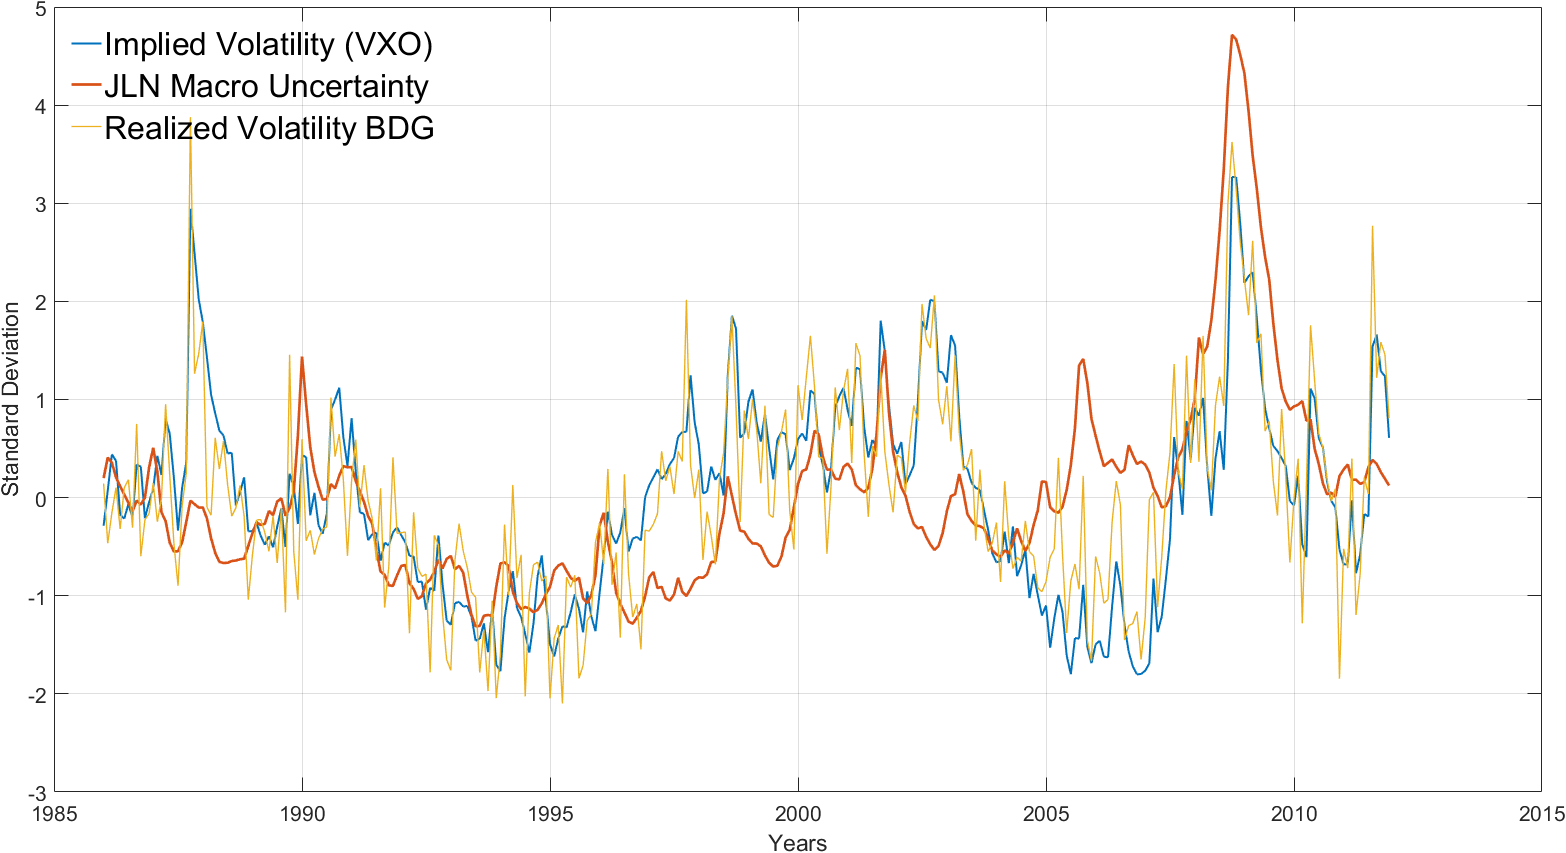
\includegraphics[scale=0.26]{Uncertainty}
		\end{center}
		
		
		\begin{center}
			\begin{tabular}{ c | c c c c}
				& VXO & JLN & BDG \\ \hline
				IP  &     -0.2358         & -0.4935         &  -0.2822    \\

			\end{tabular}
		\end{center}
		
		
	}
	
		\frame{\frametitle{Uncertainty as a driver of the business cycle}
		
		The acute instability that featured financial markets during the 2007-09 crisis and the relation with its unprecedented severity and duration have set doubts on known sources of economic fluctuations.
		
		\
		
		Since then, uncertainty has been proposed as a new potential driver of the business cycle.
		
		\
		
		Empirical literature has been called to answer the following positive questions
		
		\begin{itemize}
			\item Is uncertainty just an endogenous response to 1st-moment shocks?
			\item Does uncertainty plays an autonomous and active role as a driver of the cycle?
		\end{itemize}
		
		
	}
	
	\frame{\frametitle{Uncertainty as a theoretical concept}		
		
		\begin{itemize}
			
			\item Frank Knight in 1921 defined \textbf{uncertainty} as people's inability to forecast the likelihood of events happening.
			
			\
			
			\
		    
		    \
		    
		    \
		    
		    \item Today, uncertainty is represented by the expected volatility of the unforecastable part of key macroeconomic variables.
		    
		    \begin{itemize}
		    	\item Uncertainty $\neq$ Volatility (!)
		    \end{itemize}
		
		\end{itemize}			
}

	\frame{\frametitle{Uncertainty as an empirical measure}
	
	
\begin{itemize}
	
	\item Uncertainty cannot be directly observed
	
	\
	
	\
	
	\item A series of different proxies
	\begin{enumerate}
		\item Financial realized volatility 
		\item Financial implied (expected) volatility 
		\item Disagreement among a group of forecasters 
		\item Cross sectional dispersion of firm profits
		\item Narrative approach
	\end{enumerate}
	
	\
	
	\
	
	\item Jurado et al. (2015) provided a generalized measure of macro uncertainty which is consistent with its theoretical concept.
	
	
\end{itemize}

}	

\frame{\frametitle{Research Question}
	
	\begin{itemize}
	
\item Which is the \textbf{causal effect} of uncertainty on economic activity?	

\

\

\item In other words, which is the effect of an \textbf{uncertainty shock} on macroeconomic variables?

\

\

\item Ideally, I would like to estimate through a \textbf{semi-structural model} a series of \textit{primitive} and \textit{exogenous} changes in agents' ability to forecast economic variables.

\begin{itemize}
\item In this specific case, structural models tend to impose the result by construction. 
\end{itemize}
	
	\end{itemize}
	
}

	




	\frame{\frametitle{Main Related Literature}
		


			\begin{itemize}
				\item Stock and Watson (2012) - Brookings;
				\item Jurado, Ludvigson, and Ng (2015) - AER;
				\item Caldara, Fuentes-Albero, Gilchrist, and Zakrajsek (2016) - EER;
				\item Berger, Dew-Becker, and Giglio (2019) - R\&R REStud;
				\item Cascaldi-Garcia and Galvao (2019) - forthcoming JMCB;
				\item Ludvigson, Ma, and Ng (2017) - NBER working paper. 
				\item Carriero, Clark, and Marcellino (2019) - forthcoming REStat
				\item Carriero, Clark, and Marcellino (2018) - working paper
			\end{itemize}    
	
		
	}

	\frame{\frametitle{Challenges}
		
		\begin{enumerate}
			\item It is a \textbf{latent variable}
						\begin{itemize}
				\item it cannot be directly observed
			\end{itemize}
		
		\
			
			\item Potential \textbf{reverse-causality} with current shocks
			\begin{itemize}
				\item uncertainty responds on impact to any 1st-moment shocks
				\item aggregate variables respond on impact to uncertainty shocks
			\end{itemize}
		
		\
		
		\item Potential \textbf{endogeneity} with any news shocks
					\begin{itemize}
			\item Signal regarding future states of the economy may affect current uncertainty 
		\end{itemize} 
	

\

\item It is deeply confounded with \textbf{financial shocks}
\begin{itemize}
	\item Exogenous changes to the supply of any form of lending
\end{itemize}
	
	
		\end{enumerate}
		
	}

	\frame{\frametitle{Latent Variable}
		
		
		Exercise where VXO innovation is completely unrelated to JLN innovation
				
	}


	\frame{\frametitle{Reverse causality with current shocks}
	
	Proxy SVAR with synthetic instrument, narrative approach
	
}


	\frame{\frametitle{Endogeneity with news shocks}
	
	SPF have the right timing
	
	\
	
	Romer and Romer, and Valerie Ramey control for future signals
	
	\
	
	Robustness check for Barsky and Sims shocks but squared!
	
}

	\frame{\frametitle{Financial Shocks vs Uncertainty Shocks}
	
	Internal instrument cash flow
	
}

\end{document}